%
% SD removed as we said it earlier already
%%%(\eg  \prg{a1}.\prg{myBank} = \prg{a2}.\prg{myBank}),   %kjx elided
%%
%%
%\Chainmail\ incorporates assertions   about
%%\susan{the intro mentions viewpoint as well - the two should be consistent}
%%
%\textit{permission},
%% --- objects being accessible from other objects (\eg
%% $\CanAccess{\x}{\y}$);
%%
%\textit{control},
%% --- the next method to be invoked ($\Calls {\x} {\y} {\m} {\z}$);
%%
%%\textit{authority},
%%  --- about the change of some property (\eg $\Changes{\x.\f}$);
%%
%\textit{space}, %--- some property being observable within a subset of
%%the current state ( $\Using{\A}{S}$);
%%
%\textit{time},
%%
%and \textit{viewpoint},
%% --- about some property holding in the future or in the past (\eg $\Future \A$ or $\Past \A$).
%%
%as well as   ``classical'' assertions \sophia{would be nice iof we had a better name}
%about  variables and the heap.
%%
In this Section we  give a brief and informal  overview of some of the most salient features of  
\Chainmail -- a full exposition appears in Section \ref{sect:assertions}.



\sdparagraph{Example Configurations} We  will illustrate these features using the  \prg{Bank}/\prg{Account} example from the previous Section.
We   use the runtime configurations $\sigma_1$ and $\sigma_2$ 
shown in the left and right diagrams in Figure \ref{fig:BankAccountDiagrams}.
%These configurations could arise from the execution of different implementation of the \prg{Bank}/\prg{Account}
% module.
In both diagrams the rounded boxes depict objects:  green for those from the 
\prg{Bank}/\prg{Account} component, and grey for the ``external'',  ``client'' objects.
The transparent green rectangle  shows which objects are contained by the \prg{Bank}/\prg{Account} component.
The object at \prg{1} is a \prg{Bank}, those at \prg{2}, \prg{3} and \prg{4} are 
\prg{Account}s, and those at \prg{91}, \prg{92}, \prg{93} and \prg{94} are 
``client'' objects which belong to classes different from those from the \prg{Bank}/\prg{Account}  module.

Each configuration represents one alternative implementation of the Bank object.
Configuration  $\sigma_1$ may arise from execution using a module $M_{BA1}$, where  \prg{Account} objects
  have a field \prg{myBank} pointing to their \prg{Bank}, and an integer field  \prg{balance}
-- the code can be found in appendix~\ref{Bank:appendix} Fig.~\ref{fig:BanAccImplV1}.
Configuration  $\sigma_2$ may arise from execution using a module $M_{BA2}$,  where \prg{Account}s have a \prg{myBank}
field,  \prg{Bank} objects  have a \prg{ledger} implemented though a sequence of \prg{Node}s, each of which has a
 field pointing to an \prg{Account}, a field \prg{balance}, and a
 field \prg{next} -- the code can be found in appendix~\ref{Bank:appendix}
Figs.~\ref{fig:BanAccImplV2a} and~\ref{fig:BanAccImplV2b}.

 
 
\begin{figure}[htbp]
\begin{tabular}{cc}
 \begin{minipage}{0.45\textwidth}
$\sigma_1$\\
 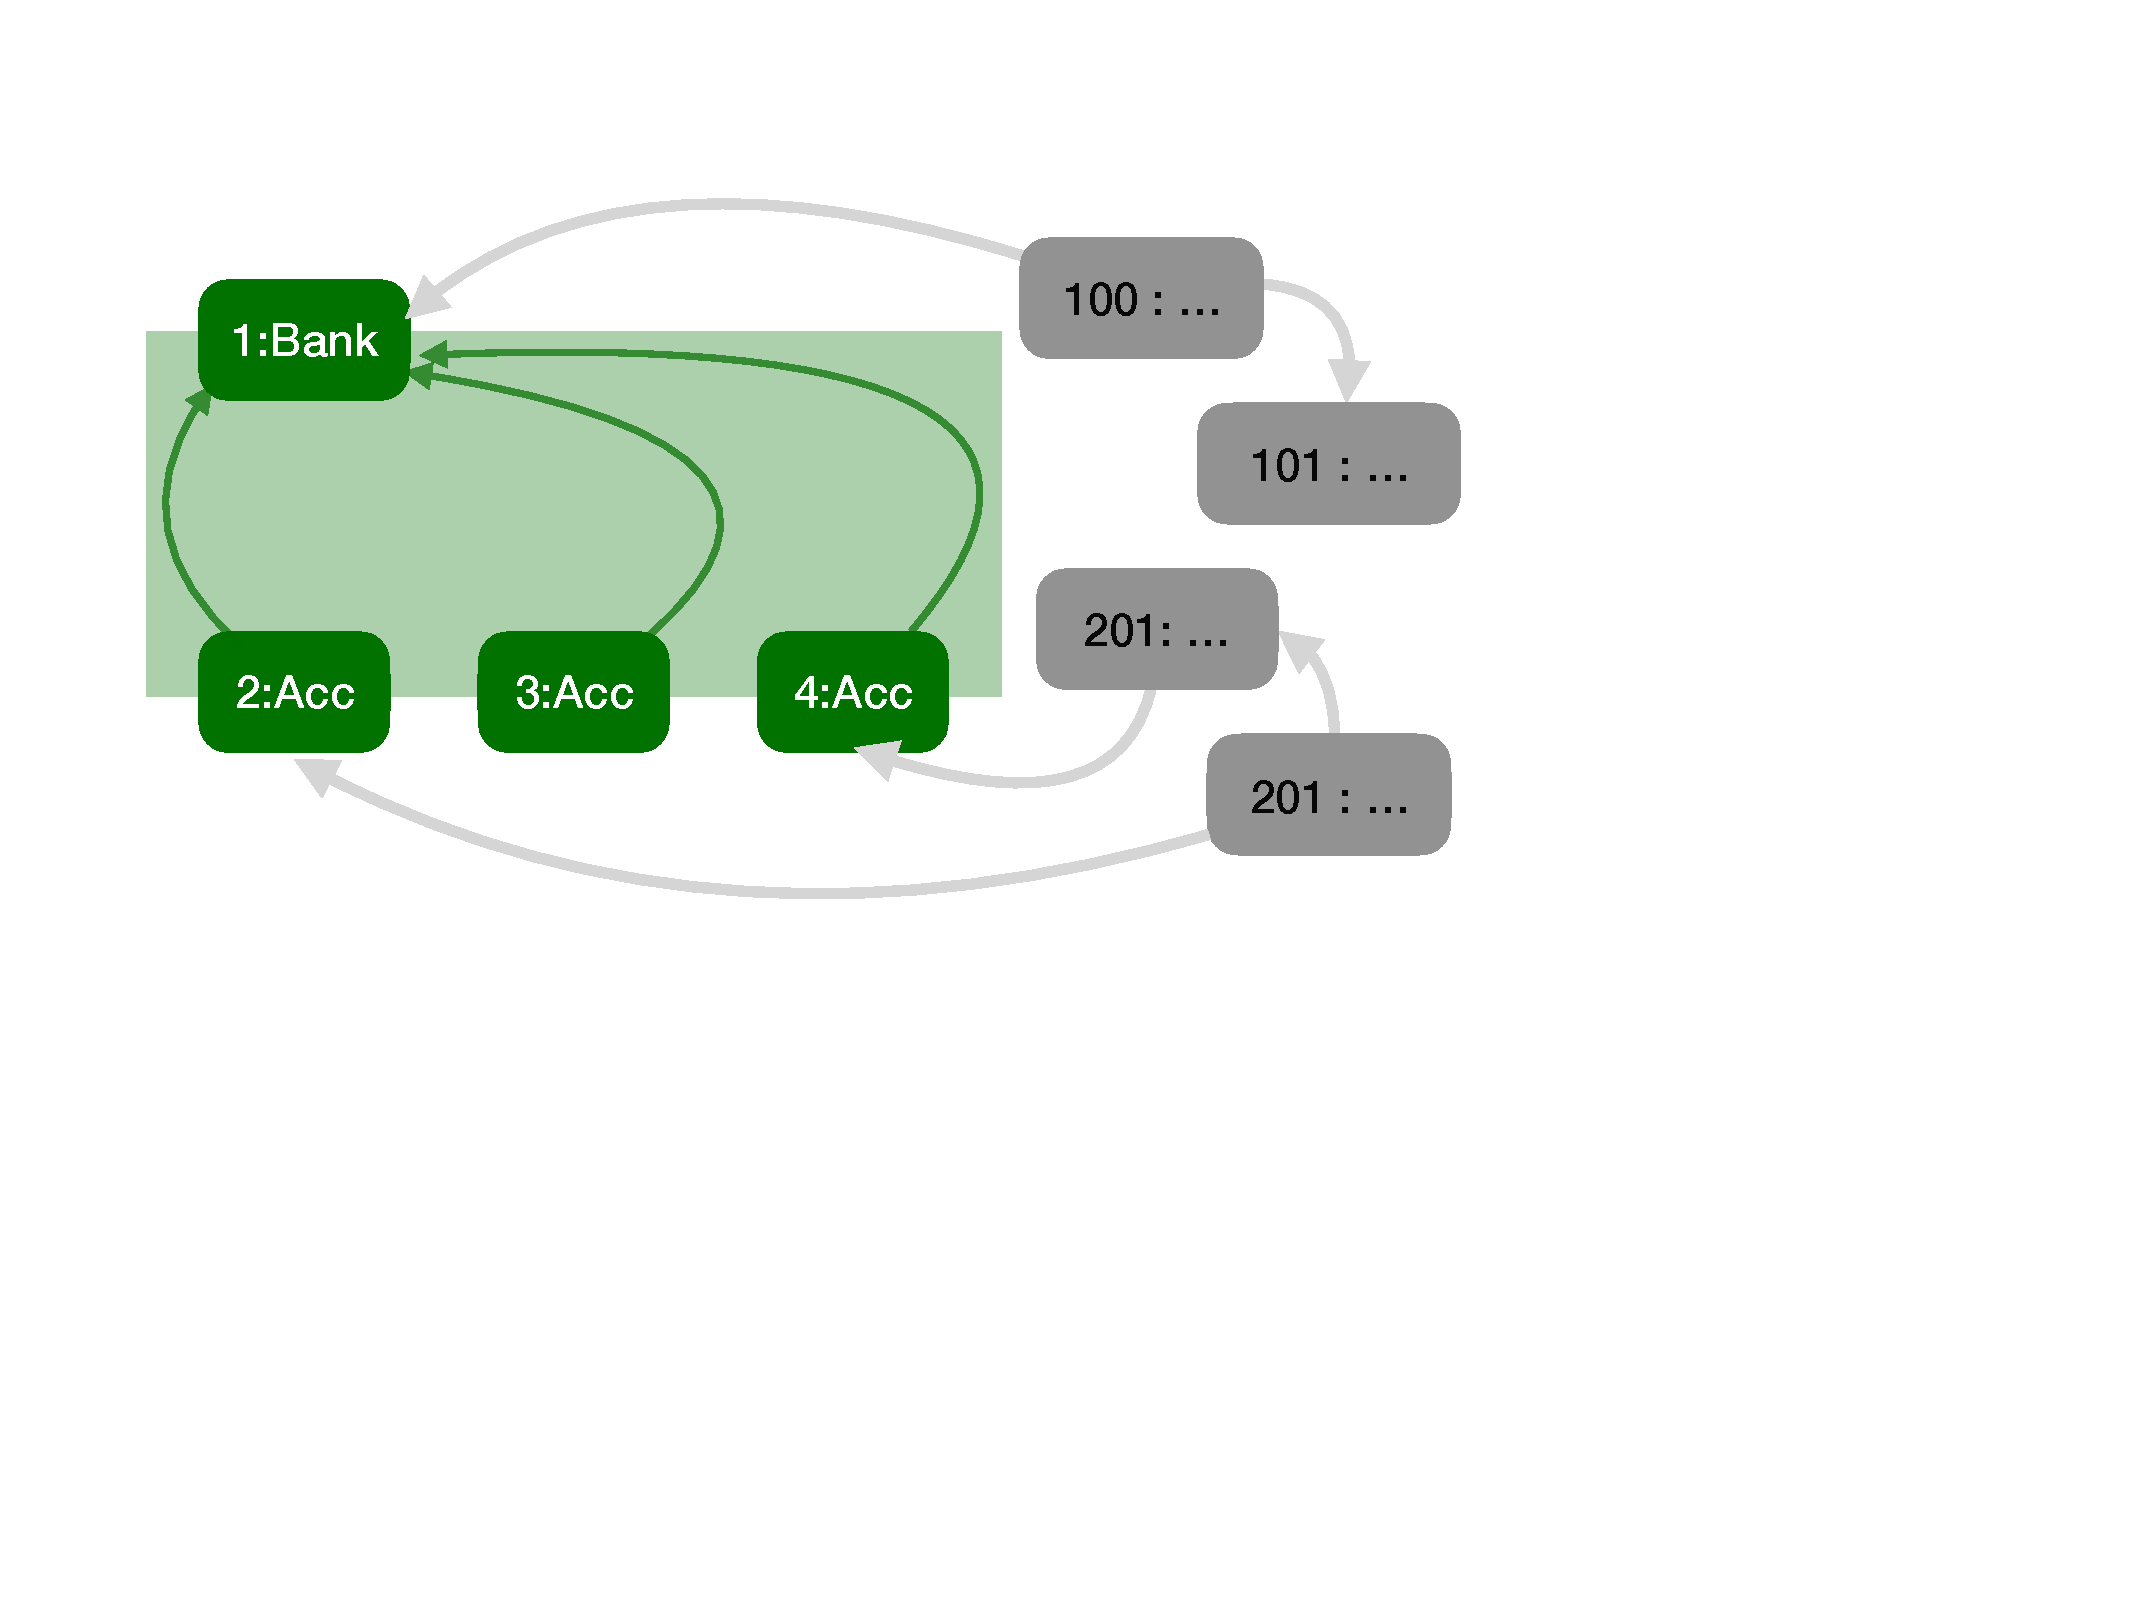
\includegraphics[width=\linewidth, trim=55  330 320 60,clip]{diagrams/BankAccount_version_1.pdf}
   \end{minipage}
 &  
 \begin{minipage}{0.45\textwidth}
 $\sigma_2$\\
  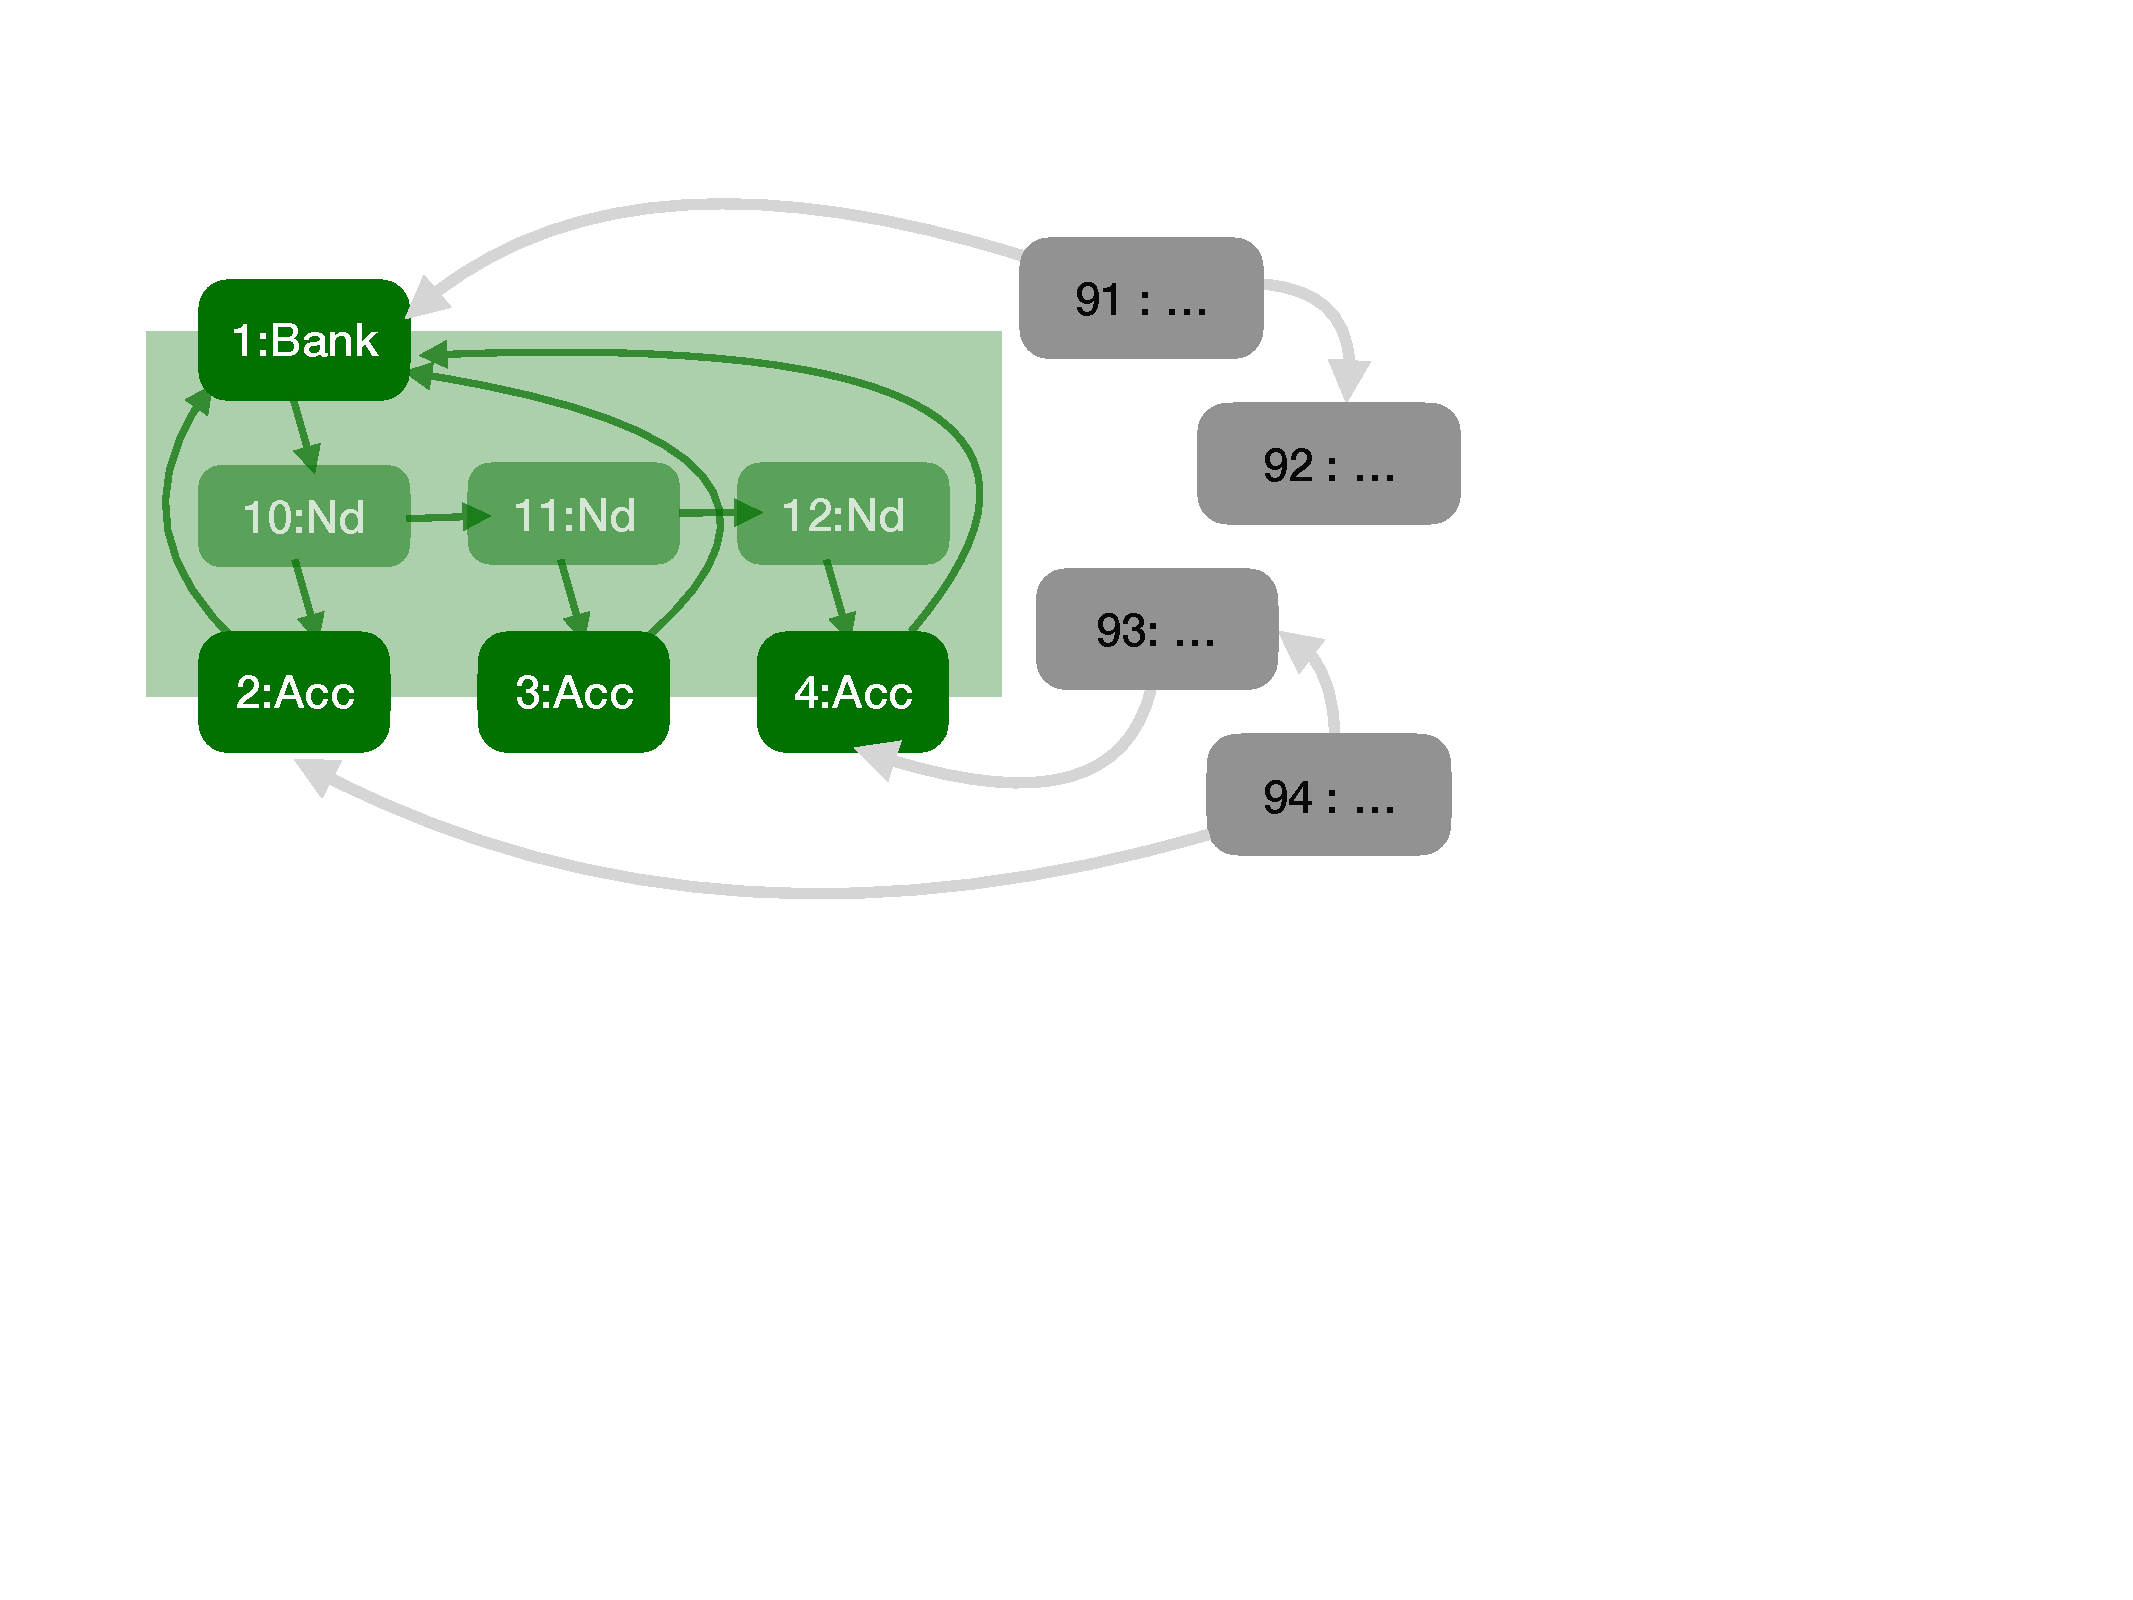
\includegraphics[width=\linewidth, trim=55  330 320 60,clip]{diagrams/BankAccount_version_2.pdf}
   \end{minipage}
\end{tabular}
\caption{Two runtime configurations for the \prg{Bank}/\prg{Account} example. 
}
\label{fig:BankAccountDiagrams}
\end{figure}

\noindent 
For the rest,  assume variable identifiers $\prg{b}_1$, and $\prg{a}_2$--$\prg{a}_4$, and  $\prg{u}_{91}$--$\prg{u}_{94}$ denoting objects \prg{1}, \ \prg{2}--\prg{4},
and   \prg{91}--\prg{94} respectively for both $\sigma_1$ and $\sigma_2$.
That is, for $i$=$1$ or $i$=$2$, $\sigma_i(\prg{b}_1)$=\prg{1}, 
$\sigma_i(\prg{a}_2)$=\prg{2}, $\sigma_i(\prg{a}_3)$=\prg{3},  $\sigma_i(\prg{a}_4)$=\prg{4},  
  $\sigma_i(\prg{u}_{91})$=\prg{91}, $\sigma_i(\prg{u}_{92})$=\prg{92},   
  $\sigma_i(\prg{u}_{93})$=\prg{93}, and $\sigma_i(\prg{u}_{94})$=\prg{94}.



\sdparagraph{Classical Assertions} talk about the contents of the 
local variables (\ie the topmost stack frame), and the 
fields of the various objects (\ie the heap).  
  For example, the assertion  $\ \prg{a}_2.\prg{myBank}$=$\prg{a}_3.\prg{myBank} $, says that
  $\prg{a}_2$ and  $\prg{a}_3$  have the same bank. In fact, this assertion is
  satisfied in both $\sigma_1$ and $\sigma_2$, written formally as\\
  $\strut$ \hspace{1.1cm}  $...,\sigma_1 \ \models \ \prg{a}_2.\prg{myBank}=\prg{a}_3.\prg{myBank}$
  \\
 $\strut$ \hspace{1.1cm}  $...,\sigma_2 \ \models \ \prg{a}_2.\prg{myBank}=\prg{a}_3.\prg{myBank}$.
   
 
  The term \prg{x}:\prg{ClassId} says that \prg{x} is an object of class \prg{ClassId}. For example\\
  $\strut$ \hspace{1.1cm}  $...,\sigma_1 \ \models \ \prg{a}_2.\prg{myBank} : \prg{Bank}$.
  
  We support ghost fields~\cite{ghost,Leavens-etal07}, 
   \eg $\prg{a}_1$.\prg{balance} is a physical field in $\sigma_1$ and a ghost field in $\sigma_2$ since in \prg{MBA2} an \prg{Account} does not store its \prg{balance} (as can be seen in appendix~\ref{Bank:appendix}
Fig.~\ref{fig:BanAccImplV2a}). %\sd{The abstract function %this is a term from the ESOP'06 paper from aboove
 % for \prg{balance}  is defined in  the body of class \prg{Account}}  in \prg{MBA2}  \sd{in the obvious way}.
%
We also support the usual logical connectives, and so, we can express assertions such as \\
$\strut$ \hspace{1.1cm}    $\forall \prg{a}. [ \ \ \prg{a}:\prg{Account} \ \longrightarrow \ \ \prg{a}.\prg{myBank}:\prg{Bank}\ \wedge\  \prg{a}.\prg{balance}\geq 0\ \ ] $ .



\sdparagraph{Permission: Access}
%
Our first holistic assertion, $\CanAccess{\x}{\y}$, asserts that  
object $\x$ has a direct reference to another object $\y$: either one
of $\x$'s fields contains a 
reference to $\y$, or the receiver of the currently executing method is \prg{x}, and \prg{y}
is one of the arguments or a local variable. 
For example:\\
 $\strut$ \hspace{1.1cm}  $...,\sigma_1 \ \models \  \CanAccess{\prg{a}_2}{\prg{b}_1}$
\\
If  $\sigma_1$ 
were executing the method body corresponding to the call ${\prg{a}_2}$.\prg{deposit}\prg{(}${\prg{a}_3}$,\prg{360}\prg{)},  then
we would 
  have\\
 $\strut$ \hspace{1.1cm}  $...,\sigma_1 \ \models \  \CanAccess{\prg{a}_2}{\prg{a}_3}$, \\
 Namely, during execution of \prg{deposit}, the object  at   $\prg{a}_2$ has access to the object at $\prg{a}_3$, and could,
  if the method body chose to,  call a method on $\prg{a}_3$ , or  store a reference to $\prg{a}_3$ in its own fields.\\
  %  \sophia{ALL: does this clarify why   we define access to take method execution into account?} 
 Aaccess is not symmetric, nor transitive:\\
  $\strut$ \hspace{1.1cm}  $...,\sigma_1 \ \not\models \  \CanAccess{\prg{a}_3}{\prg{a}_2}$, \hspace{0.6cm}\\
  $\strut$ \hspace{1.1cm} 
  $...,\sigma_2 \ \models \  \CanAccessTr{\prg{a}_2}{\prg{a}_3}$, \hspace{0.6cm}
 %   $\strut$ \hspace{1.1cm}  
 $...,\sigma_2 \ \not\models \  \CanAccess{\prg{a}_2}{\prg{a}_3}$.


%\james{do we really not also need reachable (transitive closure of access)}
%\susan{we don't seem to need transitivity in any of the examples}
%\sophia{We do not want transitivity, our policies where access is in the conclusion would become too weak.}

\sdparagraph{Control: Calls}
%
The  assertion $\Calls {\x} {\y} {\m} {\zs}$
% \sophia{it said " is more-or-less the control flow analogue of
% the access assertion" -- that is a nice simile, but is it true?\kjx{I
% think it's true}} 
 holds 
in program states where a method on object 
${\x}$ makes a method call ${\y}.{\m}({\zs})$ --- that is it calls method 
{\m} with object {\y} as the receiver, and with arguments {\zs}.
For example, \\
 $\strut$ \hspace{1.1cm}  $...,\sigma_3 \models \  \Calls {\x}{\prg{deposit}}  {\prg{a}_2} { {\prg{a}_3},\prg{360}}$.\\
 %{{...}} {\prg{a}_2}} {\prg{deposit}} {\prg{(}{\prg{a}_3},\prg{100.00}\prg{)}}$.\\
 means that the receiver in %configuration
 $\sigma_3$ is \x, and that
 $\prg{a}_2.\prg{deposit}{\prg{(}}\prg{a}_3,\prg{360}{\prg{)}}$
 is the next statement to be executed.
 

%% \sdparagraph{Authority --  Changes and Internal/External}\sophia{Is it good to put these together?}
%% The assertion $\Changes{\prg{e}}$  holds when the value of {\prg{e}}
%% in the next configuration is different to the value in the current configuration.
%% For example, if the code being executed in $\sigma_1$ started with $\acc_2.\bal=\acc_2.\bal+\prg{100.00}$, then:\\
%%   $\strut$ \hspace{1.1cm}  $..., \sigma_1 \ \models \  \Changes {\acc_2.\bal}$.\\
%%   Moreover, the assertion $\External {\prg{e}}$ expresses that the object {\prg{e}} does not belong to the module under consideration. 
%%   For example, \\
%% $\strut$ \hspace{1.1cm}  $\M_{AB2}\mkpair ..., \sigma_2 \ \models \ \External{\pu_{92}}$,
%% %$\strut$ 
%% \hspace{1cm}  $\M_{AB2}\mkpair ..., \sigma_2 \ \not\models \ \External{\acc_2}$, \\
%% $\strut$
%%  \hspace{1.1cm}  $\M_{AB2}\mkpair ..., \sigma_2 \ \not\models \ \External{\pb_{1}.\prg{ledger}}$\\
%% Notice the use of the \emph{internal} module, $\M_{AB2}$, needed to judge which objects are internal, and which are external.
 

\sdparagraph{Space: {In}}
The space assertion $\Using{\A}{\SF}$ establishes validity of $\A$ 
 in a configuration  restricted to the 
objects from the set \SF.
% In other words, it restricts the set of objects which may be used to establish property \A. 
For example, 
if  object \prg{94}  is included in $\SF_1$ but not in  $\SF_2$, then we   have\\ 
 $\strut$ \hspace{1.1cm}  $..., \sigma_1 \ \models \ \Using{ (\exists \prg{o}.\,\CanAccess{\prg{o}}{\acc_4})}{\SF_1}$
\\ % $\strut$ \hspace{0.2cm}  
 $\strut$ \hspace{1.1cm}  $..., \sigma_1 \ \not\models \ \Using{ (\exists \prg{o}.\,\CanAccess{\prg{o}}{\acc_4})} {\SF_2}$.\\
 The set \SF\ in the assertion $\Using{\A}{\SF}$  is therefore {\em not} the footprint of   $\A$;
  it is more like the \emph{fuel}\cite{stepindex}  given to establish that assertion. Note that  $..., \sigma \ \models \Using {\A} {\SF}$ does not imply  
  $..., \sigma \ \models \A$  nor does it imply   $..., \sigma \ \models \Using {\A} {\SF\cup\SF'}$.
  The other direction of the implication does not hold either.
% \james{would still like  a one sentence motivating/justifying ``with''. Why do we need it}

\sdparagraph{Time: Next, Will, Prev, Was}
We support several operators from temporal
logic: ($\Next \A$, $\Future \A$,  $\Prev \A$, and $\Past \A$) to
talk about the future or the past in one or more number steps.
The assertion $\Future \A$ expresses that %after one or more execution steps
$\A$ will hold in one or more steps. For example, 
taking $\sigma_4$ to be similar to  $\sigma_2$, the next statement to be executed 
to be  $\prg{a}_2.\prg{deposit}{\prg{(}}\prg{a}_3,\prg{360}{\prg{)}}$, and 
$\M_{BA2}\mkpair ..., \sigma_4 \ \models \  \acc_2.\bal=\prg{60}$,  and that
$\M_{BA2}\mkpair ..., \sigma_4 \ \models \  \acc_4.\bal\geq\prg{360}$,
then\\ 
 $\strut$ \hspace{1.1cm}  $\M_{BA2}\mkpair ..., \sigma_4 \ \models \ \Future{ {\acc_2.\bal}=\prg{420}}$.\\
The \emph{internal} module, $\M_{BA2}$ is needed for looking up the method body of \prg{deposit}.
  
\sdparagraph{Viewpoint: --  External}
%% The assertion $\Changes{\prg{e}}$  holds when the value of {\prg{e}}
%% in the next configuration is different to the value in the current configuration.
%% For example, if the code being executed in $\sigma_1$ started with $\acc_2.\bal=\acc_2.\bal+\prg{100.00}$, then:\\
%%   $\strut$ \hspace{1.1cm}  $..., \sigma_1 \ \models \  \Changes {\acc_2.\bal}$.\\
The assertion $\External {\prg{x}}$ expresses that the object at {\prg{x}} does not belong to the module under consideration. 
  For example, \\
$\strut$ \hspace{1.1cm}  $\M_{AB2}\mkpair ..., \sigma_2 \ \models \ \External{\pu_{92}}$,
%$\strut$ 
\hspace{1cm}  $\M_{AB2}\mkpair ..., \sigma_2 \ \not\models \ \External{\acc_2}$, \\
$\strut$
 \hspace{1.1cm}  $\M_{AB2}\mkpair ..., \sigma_2 \ \not\models \ \External{\pb_{1}.\prg{ledger}}$\\
The \emph{internal} module, $\M_{BA2}$, is needed to judge which objects are internal or external.
 
\sdparagraph{Change and Authority:} We have used 
$\Changes {...}$ 
in our \Chainmail assertions in section~\ref{sect:motivate:Bank}, as in
 $\Changes  {\acc.\prg{balance}}$. Assertions that talk about change, or give conditions for change
to happen are fundamental for security; the ability to cause change is called \emph{authority} in \cite{MillerPhD}. 
We could encode change using the other features of \Chainmail, namely, for any expression \e:\\
$\strut$ \hspace{1.1cm}
$\Changes {\e}$\  \ $\equiv$\ \ $\exists v. [\ \e=v \wedge \Next {\neg ( \prg{e}=v)}\ ]$.\\
and similarly for assertions.


%\sophia{The observer pattern example is very nice, but unfortunately we cannot use it, because the
%calls are internal, and therefore not visible in the current system.}
%For example, a part of the observer pattern is that when
%a subject is notified of a change, then the observer must
%be told to update itself.    We can write this from the
%subject's perspective, looking forwards:
%
%\begin{lstlisting}
%  Call(_,subject,notify,_) --> Will(Call(subject,observer,update,_))
%\end{lstlisting}
%
%\noindent meaning that once notify is called on a subejct, then its
%observer will be updated sometime in the future.  We can write a very
%similar specification for an observer, looking backwards.
%
%\begin{lstlisting}
%  Call(subject,observer,update,_) --> Was(Call(_,subject,notify,_))
%\end{lstlisting}
%
%\noindent meaning that if a subject updates an observer, that subject
%have been notified sometime previously. We could tighten each
%specifaction, so that the update must immediately follow the
%notification, by replacing $\Future \A$ or $\Past \A$ with 
%$\Next \A$ or $\Prev \A$.

\sdparagraph{Putting these together} We now look at some composite assertions which use  
 several features from above. The assertion below 
says that if the statement to be executed is   $\acc_2.\prg{deposit}\prg{(}\acc_3,\prg{60}\prg{)}$,
then the balance of $\acc_2$ will eventually change:\\
 $\strut$ \hspace{1.1cm}  
 $\M_{BA2}\mkpair ..., \sigma_2 \ \models \ {\Calls {..}   {\prg{deposit}} {\acc_2} {\acc_3,\prg{60}} } \longrightarrow {\Future{ \Changes {\acc_2.\bal}}}$.

\vspace{.2cm}
 
Now look deeper into   space assertions, $\Using{\A}{\SF}$: They allow us to characterise the set of objects which have authority over certain effects (here $\A$). In particular,  the assertion   $\Using {\Future {\A}} {\SF}$  requires two things: i) that $\A$ will hold in the future, and ii)  that the objects which cause the effect which will make $\A$ valid, are   included in \SF.
Knowing who has, and who has not, authority over properties or data is a fundamental concern of robustness
\cite{MillerPhD}. Notice that the authority is a set, rather than a single object: quite often it takes \emph{several objects in concert}
 to achieve an effect.


Now, consider assertions (2) and (3) from the previous section. They both have the form\\
 $\strut$ \hspace{1.1cm}  $\Future {\Using {\A} {\SF}}\ \longrightarrow P(\SF)$,\\
  where $P$ is some property over a set. These assertion say, that if ever in the future $\A$ becomes valid, and if the objects involved in making $\A$ valid are included in $\SF$, then $\SF$ must satisfy $P$. Such assertions can be used to restrict whether $\A$ will become valid. Namely, if we have some execution which only involves objects which do not satisfy $P$, then we know that the execution will not ever make $\A$ valid.

%\susan{I don't know where m and m2 come from. We haven't seen them up to now and I don't  see why they are needed in this story.}

%%\vspace{.2in} 
%\sophia{While
%many  individual
%features of \Chainmail can  be found also in other work, we
%%claim that their  combination as well as
%%their application in the specification of open systems are novel.
%argue that their power and novelty for specifying open systems lies in their careful
%  combination}
 
\sdparagraph{In summary,} in addition to classical 
logical connectors and classical assertions over the contents of the heap and the stack, 
our holistic assertions draw from some concepts from object capabilities
($\CanAccess{\_}{\_}$  for  permission; {$\Calls {\_} {\_} {\_} {\_}$ and  $\Changes{\_}$ for
authority) 
as well as temporal logic ($\Future \A$, $\Past \A$ and friends), and the relation of
our spatial connective ($\Using{\A}{S}$)  with ownership and effect
systems \cite{typeEffect,ownalias,ownEncaps}.

The next two sections  discuss the semantics of \Chainmail. Section \ref{sect:formal}
contains an overview of the formal model and section \ref{sect:assertions} focuses on the most important part of \Chainmail : assertions.

%its most important aspect being assertions, whose semantics are in section  \ref{sect:assertions}.

%\james{somewhere, should we say something like: the goal is
%  to allow wholistic specifations with as extra little machinery as
%  possible over a basic Hoare language}.


